% Template v2.0: 11/13/2018.   The previous template is also acceptable. 
% Template for white paper submissions for the 
% LSST Call for Observing Strategies for DeepDrilling and Minisurveys 
% 
% The call for white papers can be found at https://github.com/lsst-pst/survey_strategy/blob/master/latex/WPcall2018.pdf
% The deadline for submissions is November 30, 2018
% To submit white papers, please email the compiled PDF to lsst-survey-strategy@lists.lsst.org   
%  OR submit a pull request to this github repository (github.com/lsst-pst/survey_strategy_wp) with your white paper in a clearly named subdirectory.
% For help with white papers or the submission process, please post at http://community.lsst.org/c/sci/survey-strategy


\documentclass[12pt, letterpaper]{article}
\usepackage[top=1in, bottom=1.5in, left=1in, right=1in]{geometry}
\usepackage[utf8]{inputenc}
\usepackage{booktabs}
\usepackage{hyperref}

\usepackage[english]{babel}
\usepackage{amsmath}
\usepackage{amssymb}
\usepackage{graphicx}
\usepackage{hyperref}
\usepackage{wrapfig,verbatim,caption,subcaption,calc,relsize,multicol,enumitem,titlesec}

\usepackage[utf8]{inputenc}
\usepackage{booktabs}
\usepackage[utf8]{inputenc}
\usepackage{natbib}

%Includes "References" in the table of contents
\usepackage[nottoc]{tocbibind}
\def\apj{AstroPhysical Journal}             % Astrophysical Journal
\def\apjl{Astrophysical Journal, Letters}                % Astrophysical Journal, Letters
\def\apjs{Astrophysical Journal, Supplements}  \def\nat{Nature}               % 
\def\mnras{Monthly Notices of the Royal Astronomical Society}
\newcommand\mathmacro[1][A]{\ensuremath{{#1}_1}}

%%% macroe %%%
\newcommand{\dtone}{\ensuremath{\Delta T_1}}
\newcommand{\dttwo}{\ensuremath{\Delta T_2}}
\title{Explosive Physics \& Fast Transients LSST Cadence}
\author{\small{Federica B. Bianco\footnote{fbianco@nyu.edu}, NYU CUSP/CCPP NYU, University of Delaware;}\\\small{Melissa Graham, University of Washington;}\\\small{Igor Andreoni, Caltech; Rahul Biswas, Stockholm University Philip Cowperthwaite,}\\\small{Carnegie; Maria Drout, Dunlap Institute, University of Toronto;}\\\small{Gautham Narayan, STScI; Tyler A Pritchard, NYU; Tiago Ribeiro, LSST; 
}}
\date{\today}

\begin{document}

\maketitle

\begin{abstract}
We propose a cadence for the LSST survey in which three visits are obtained per night: two different filters within a short time window (e.g., $g$ \& $i$ or $r$ \& $z$ within $\sim1$ hour) and a repeat of one of those filters with a longer time window (e.g., $\sim4$ hours). We colloquially refer to this as the {\em Presto-Colores} strategy (quick-colors). This observing strategy delivers both the color and lightcurve evolution of transients on the same night. This will enable us to identify and characterize fast transients -- or fast features of longer timescale transients -- such as rapidly-declining supernovae (SNe), kilonovae (KNe), and the signatures of SN ejecta interacting with binary companion stars or circumstellar material. Such extragalactic transients are intrinsically rare, thus LSST could dramatically improve our understanding of their origin and properties. This cadence can be implemented as a Mini-Survey or as part of a Wide-Fast-Deep survey on selected portions of the extragalactic sky.
\end{abstract}

\section{White Paper Information}
\begin{enumerate} 
\item {\bf Science Category:} Exploring the Transient Sky, Dark Energy
\item {\bf Survey Type Category:} 
We are proposing this cadence as a variation of the  `wide-fast-deep' (WFD) Main Survey, but it could also be considered for implementation as a Mini-Survey or a Deep Drilling Field, observing only a portion of the sky. 
\item {\bf Observing Strategy Category:} 
   a specific observing strategy to enable specific time domain science, that is relatively agnostic to where the telescope is pointed. 
\end{enumerate}  


\clearpage
%%%%%%%%%%%%%%%%%%%%%%%%%%%%%%%%%%%%%%%%%%%%%%%%%%%
\section{Scientific Motivation}

The advent of wide-field time domain surveys has revolutionized the field of transient astrophysics. Coverage on \emph{short timescales}, in particular, has faciliated rapid strides in our understanding of both supernova (SN) explosions and peculiar transients. Observations of ``infant'' SN---obtained hours to days after explosion---provide vital constraints on their explosion mechanisms and progenitor systems. The emission at these epochs contains natal information about the progenitor characteristics [1-4], potential non-spherical behavior [5-6], and shock collision with a binary companion [7]. In addition, rapidly-evolving transients ($\lesssim$10 days) may be associated with a variety of poorly-understood events, including accretion-induced white dwarf collapse [8], underluminous and fallback SN [9], ultra-stripped SN [10-12], compact-object mergers [13,14], orphan GRB afterglows [15], and common-envelope ejections [X].

%Do need to emphasize a bit about rates, or make it clear that 
%Need to mention ''fast features'' somewhere. They use that language. 

Despite progress, the detection rate for both rapid transients and rapidly-evolving \emph{phases/features} in SN explosions has remained low---due to a combination of survey efficiency and intrinsic event rates. The volume surveyed by LSST brings the promise of detecting many more intrinsically rare events. However, \emph{using} these events to probe the science questions described herein requires adequate time- and filter-sampling of relatively short-lived events---sampling that will \emph{not} be achieved through the WFD survey alone. Thus, we require a cadence that allows us to effectively \emph{recognize} young and rapidly-evolving transients from within millions of LSST alerts in order to trigger additional follow-up. Such a cadence has two requirements: (1)~observations in two filters obtained in quick succession so that color can be measured, and (2)~a same-filter revisit within hours so the light-curve behaviour can be analyzed and distinguished from slower-evolving transients. 

%More information on each of these: 
%Light curve rise critical to distinguish from standard SN.
%Color: critical for initial classification.

As we will show, the WFD baseline survey's inter-night revisit rate of once every three nights is too sparse, and the intra-night revisit rate of $\sim$30 minutes is too rapid, to detect \enph{and recognize} fast transients/features. The exact form of our proposed cadence is given in Section 3. In order to define our diagnostics we have selected four exemplar types of extragalactic fast transients/features. Color and rate-of-change information for each type of transient is provided in Table 1, and main science cases are discussed below.

\medskip


%\smallskip

\noindent {\bf I. The Nature of Rapidly-Evolving Luminous Transients:} ``Rapidly-evolving transients'' are defined as extragalactic events that reach SN luminosities but have timescales an order of magnitude faster [X]. To date, only a small number have been identified, but recent studies [31] have shown that they represent a significant channel ($\sim$5--10\% of the core-collapse rate) which we must understand to have a complete picture of stellar death. Known events have rise times spanning 1--3 days and blue colors at maximum  [x]. Leading theoretical models range from black hole formation to the birth of binary neutron star systems and recent observations of AT2018cow show evidence for a central engine [X,X]. More observations are required to understand their true nature and diversity. 
%They are luminous, blue, 

%More events are required to determine the nature and 
%However, these transients .

% [10,11,30], but recent studies [31] have shown that they are not \emph{intrinsically} rare---few have been detected simply because previous surveys were not designed to be efficient at short timescales. 
%with leading theoretical models including black hole formation and the birth of binary neutron star systems [5-8]

\smallskip
\noindent {\bf II. Kilonovae and the Origin of Heavy Elements:} 
Kilonova (KN) are produced by the radioactive decay of r-process nuclei synthesized in the ejecta of neutron star mergers [X].  Observations of the KN associated with GW170817 revealed thermal emission that rose in $<$ 1 day and cooled from a temperature of $>$10,000K to 3,000K over 5 days, followed by a longer-lived IR transient [X]---consistent with the production of a signifcant quantity of of r-process elements of \emph{multiple} compositions.  Additional examples---with or without associated LIGO triggers---are required to ascertain the ``typicalness'' of GW170817, with the frequency of early blue emission providing critical constraints on the ratio of light and heavy elements formed, and therefore the total contribution of NS mergers to cosmic nucleosynthesis. 
%Ejecta composition and quantity strongly influences the resulting \emph{color}, \emph{magnitude}, and \emph{timescale} of the emission.

\smallskip
\noindent {\bf III. Progentiors and Pre-explosion Mass Loss of Core-Collapse SN:} Early observations of core-collapse SN (CCSN) provide critical constraints on the progenitor radius and envelope structure through the detection of either shock breakout ($\sim$1 day) or cooling envelope ($\sim$1-4 day) emission. Indeed, in recent years, there has been growing evidence that many CCSN either explode in ``non-standard'' evolutionary states or undergo enhanced pre-SN mass-loss and outbursts in their terminal years [23,X,X]. Theoretical studies have pointed to a range of potential explanations to accommodate the observations, such as pulsation-driven superwinds [24], wave heating outbursts [25], and inflated progenitor envelope [26]. However, the nature of this mass loss and the types of SN experiencing it remain uncertain.



\smallskip
\noindent {\bf IV. Progenitors and Explosion Mechanisms of Thermonuclear SN:}
Type Ia SN result from the thermonuclear distruption of a CO white dwarf [18]. However, questions remain regarding the nature of their binary companions. Recently, observations of SN2017cbv obtained within $\sim$1 day of explosion revealed a rapidly-rising blue ``bump'', interpreted by some as a collision with a non-degenerate companion [19], while preliminary population studies reveal an as-yet-unexplained red/blue color dichotomy in the early ($<$ 5 days) rising light curves of Type Ia SN [X], with implications for outwardly mixed radioactive material predicted by the double detonation explosion model [X]. Further observations are required to ascertain the nature of this early emission, with implications from stellar physics to cosmology. 




\smallskip
\noindent {\bf V. Additional Science Cases:} While we have focused on extragalactic fast transients here, a cadence that allows measurement of both color and rate-of-change on the timescale of $\sim$hours will have general applicability across many areas---from variable stars to microlensing.

\medskip
Finally, though we describe here an adaptation to the general WFD cadence to facilitate the timely identification of rapid events, our cadence could alternatively be adopted as a mini-survey over a portion of the sky. If coupled with a shorter intra-night cadence (as part of a mini-survey or due to a rolling candence) LSST observations alone could provide sufficient light curve coverage to probe progenitors and explosion physics of fast transients/features.

\bigskip

\noindent {\bf MRD Note: I'm still working to clean this up and cut some text. A few things could move to later sections. Ah, we now have more room! I will expand a few things slightly and fix the references.}

\clearpage
%%%%%%%%%%%%%%%%%%%%%%%%%%%%%%%%%%%%%%%%%%%%%%%%%%%%%%%%
%%%%%ORIGINAL MOTIVATION:
%%%%%%%%%%%%%%%%%%%%%%%%%%%%%%%%%%%%%%%%%%%%%%%%%%%%%%%%%


%\begin{footnotesize}
%{\it Describe the scientific justification for this white paper in the context of your field, as well as the importance to the general program of astronomy, including the relevance over the next decade. Describe other relevant data, and justify why LSST is the best facility for these observations. (Limit: 2 pages + 1 page for figures.)}
%\end{footnotesize}

%%% MLG deleted text
% This has an especially high impact in two cases: (1) the relatively short-duration late stages of stellar evolution where the star undergoes rapid changes in the lead up to a supernova, and (2) binary (or even tertiary) systems where dynamical evolution and/or mass transfer plays a key role in determining the stellar evolutionary processes and outcomes. 

%{\bf note: the figures are place holders. original figures are in the making. the metrics described below are being written and optimal/feasible ranges for the parameters \dtone and \dttwo for different filter pairs will be investigated for a few science cases.}

%Explosive and eruptive transients that rise and fall in brightness within $3$--$5$ days have historically been rarely discovered due to sky survey efficiencies, but are also intrinsically rare ($\sim 5\%$ of the rate of core-collapse supernovae; \citealt{2014ApJ...794...23D}). Similarly, {\it fast features} in otherwise slow evolving transient events, such as ejecta impacting circumstellar material or a binary companion star in stellar explosions, are rarely caught due to their short-lived nature, and also appear to be intrinsically rare. Fast transients and fast features in transients provide a unique window on the physical mechanisms and progenitor scenarios of stellar eruptions and explosions, and the late stages of stellar evolution including mass-loss and mass-transfer in binaries.

%The volume surveyed by LSST brings the promise of finding and characterizing many more intrinsically rare events, however, adequate time- and filter-sampling of relatively short-lived events is necessary to deliver on this promise. The requisit observations in order to find \emph{and recognize} these fast events early enough to trigger follow-up, {\it and/or} characterize a large sample of fast events with LSST photometry alone, are: (1) observations in two filters obtained in quick succession so that color can be measured, and (2) a same-filter revisit within hours so the light-curve behaviour can be analyzed. As we will show, the WFD baseline survey's inter-night revisit rate of once every three nights is too sparse, and the intra-night revisit rate of $\sim30$ minutes is too rapid, to identify (\emph{i.e.} detect and recognize) fast transients and fast features. The exact form of our proposed cadence is given in Section 3. To define our diagnostic we collect the early-time observer-frame color and rate of change of brightness for four exemplar types of extragalactic fast transients and fast features in Table 1, discuss the main science goals for each type of transient below, and provide illustrative examples in Figure 1.

%{\bf Fast Transients --} First discovered in PanSTARRs data by \cite{2014ApJ...794...23D}, also called rapidly fading supernovae (RFSNe), and thought to be driven by the shock of low-mass ejecta propagating through an extended stellar envelope or wind (e.g., \citealt{2018MNRAS.475.3152K}). There are only tens of such RFSNe discovered so far. The sample presented in \cite{2014ApJ...794...23D} mostly have $z<0.3$, rise to peak within $1$--$3$ days (e.g., PS1-10bjp rises by $2.2$ mag in $g$-band during the $2.7$ days before peak), and are optically blue (observer-frame; figure 9 of \citealt{2014ApJ...794...23D}).

%{\bf Kilonovae --} The discovery of kilonovae, whether or not they are associated with LIGO events, yeilds new insights into neutron star mergers. The optical counterpart to GW170817 presented by \cite{2017ApJ...848L..27T} shows a $<2$-day rise to peak brightness, at which point the color $r-Y\sim0.5$, after which the emission evolves redward (e.g., their figure 3) and declines quickly (e.g., $6$ mag in $\sim10$ days; their figure 2, but see also \cite{2017Natur.551...75S}). Optical data fit with theoretical models leads to contraints on the ejecta mass and velocity and the radioactive power source.

%{\bf Core Collapse Supernova Shock Breakout --} When the shock of the core collapse reaches the photosphere, high energy emission escapes in a short luminous burst (as theoretically predicted by, e.g., \citealt{1978ApJ...223L.109K}). The serendipidous discovery of nearby ($24.6$ Mpc) SN\,2016gkg's $\sim3$-day long shock-driven feature, which in it's first day exhibted a maximum rise rate of $\sim40$ $\rm mag\ day^{-1}$, is one of the best examples to date (\citealt{2018Natur.554..497B}; see also SN\,2011dh, \citealt{2011ApJ...742L..18A}). Observations of the shock breakout can directly constrain the star's radius and the mass in its envelope. While expected to be quite blue during the initial fast rise, the optical color can be neutral or even red during the $\lesssim 3$ day shock cooling phase, e.g., $B-V\sim0.5$ for SN\,2016gkg \citep[see their extended data table 3][]{2018Natur.554..497B}.
% or $g-r\sim-0.1$ for SN\,2001dh (Arcavi et al. 2011)
% by converting the g and R on the first day
% to g-r~-0.1 via Lupton (2005) http://www.sdss3.org/dr8/algorithms/sdssUBVRITransform.php#Lupton2005
% which really isn't that appropriate

%{\bf SNe\,Ia --} Blue bumps in the first hours/days of the SN\,Ia light curve are theoretically predicted to be the photometric signature of the SN\,Ia ejecta shocking a non-degenerate companion star \citep{2010ApJ...708.1025K}, and are best exemplified with observations of SN\,2017cbv by \cite{2017ApJ...845L..11H}. The values in Table \ref{tab:1} for normal and blue bump SNe\,Ia are for nearby ($<10$ Mpc) events, derived using the $UBVgri$ photometry for SN\,2017cbv and SN\,2011fe from \cite{2010ApJ...708.1025K} within the first day of observations (see their figures 1 and 2; $U-B$ is used as a substitute $g-r$, and there was no early-time $z$ or $y$ for these events). In this case, an new point source next to an elliptical galaxy rising at $>1$ $\rm mag\ day^{-1}$ with a $g-r < -0.5$ would be an excellent candidate for a blue-bump SN\,Ia and should receive immediate follow-up. %Furthermore, obtaining color and observations within the first $\sim5$ days after explosion would enable the creation of a sample able to set constraints on the fraction of SN\,Ia originating from Single Degenerate {\it vs} Double Degenerate progenitors (as done in \citealt{Bianco2011} and indicated in \citealt{COSEP} Section 6.3), with implications for stellar physics and cosmology (as SN\,Ia may follow different standardization rules for different progenitors, inducing systematics in cosmological inference).
%Furthermore, such LSST early-time photometry and color data for SNe\,Ia could be stacked over all events, and enable statistical constraints on the fraction of SNe\,Ia that exhibit blue bumps (i.e., have non-degenerate companion stars), as done by \citealt{Bianco2011} and as indicated in Section 6.3 of \citealt{COSEP}. The types of companion stars of carbon-oxygen white dwarfs that explode as SNe\,Ia has implications for stellar physics and cosmology.

% {\bf Point-Ia --} 

% {\bf IIb+CSM --}

% {\bf Accretion-Induced Collapse (AIC) --} of a white dwarf to a neutron star,  \cite{2010MNRAS.409..846D} show they last $\sim3$ days and rise within $\sim0.5$ days to a peak R-band luminosity of $10^{41}$ $\rm erg\ s^{-1}$, which is $M_R\sim -16$ mag. {\bf MLG: Fig 2 shows their color evolution.}

\clearpage

\begin{footnotesize}
\begin{center}
\title{The early-time colors and rise rates of fast transients/features.}\label{tab:1}
\begin{tabular}{|c|c|c|} 
\hline
Target Type         & $g$-band $dm/dt$ [$\rm mag\ day^{-1}$] & color [$\rm mag$] \\
\hline 
fast transients     & $\gtrsim-0.8$ & $g-r\leq-0.2$  \\ 
kilonovae           & $>11$          & $r-Y\sim0.5$  \\ 
CCSN shock breakout & $\sim-10$     & blue at $<1$ day, then neutral  \\ 
SNIa blue bumps     & $\gtrsim -1$  & $u-g\sim-0.6$, $g-r\sim-0.2$  \\ 
SNIa normal         & $\sim -1$     & $u-g\sim-0.2$, $g-r\sim-0.1$  \\
%point-Ia (Bildsten) &  &  &  &  &  & \\ 
%IIb+CSM &  &  &  &  &  & \\ 
%AIC &  &  &  &  &  & \\ 
\hline
\end{tabular}
\end{center}
\end{footnotesize}

\begin{center}
\begin{figure}[!h]
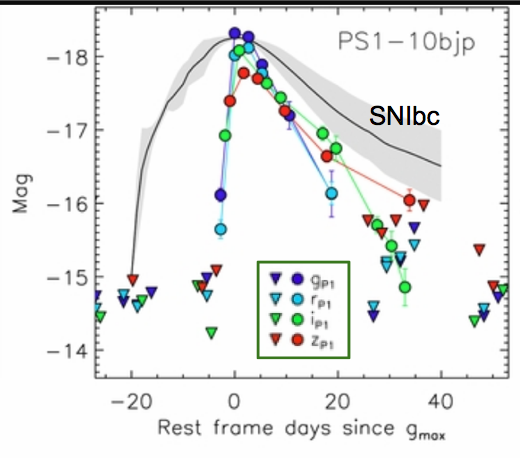
\includegraphics[width=6cm,height=5cm]{figures/Drout_PS1-10bjp.png}
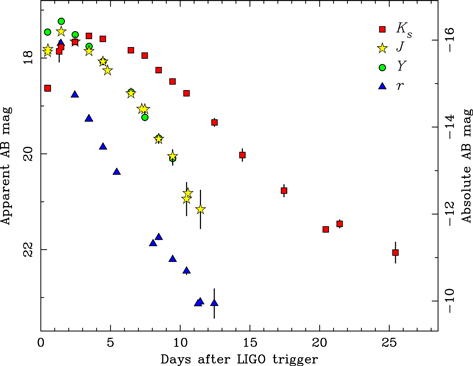
\includegraphics[width=6cm,height=5cm]{figures/Tanvir_fig2.jpg}
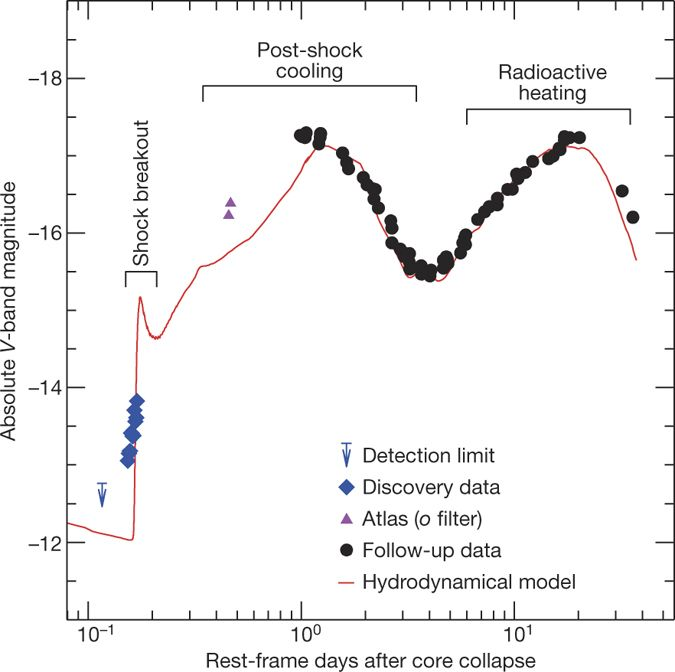
\includegraphics[width=6cm,height=5cm]{figures/Bersten_16kgk.jpg}
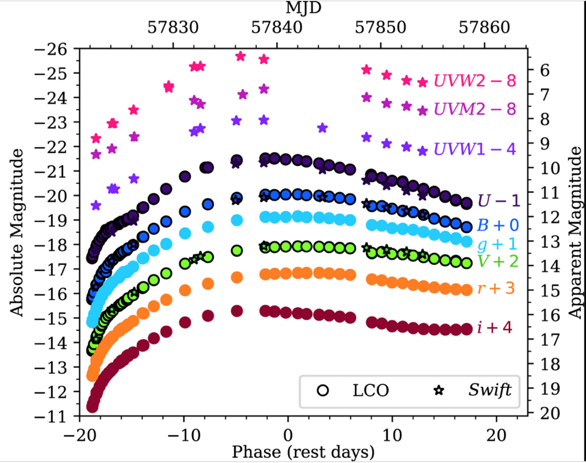
\includegraphics[width=6cm,height=5cm]{figures/Hosseinzadeh_17cbv.png}
\caption{Light curves for our examples of fast transients and fast features. Top left: Fast transient PS1-10bjp \citep{2014ApJ...794...23D}. Top right: Kilonovae for GW170817 \citep{2017ApJ...848L..27T}. Bottom left: Shock breakout for SN\,2016kgk \citep{2018Natur.554..497B}. Bottom right: SN\,Ia 2017cbv's blue bump \citep{2017ApJ...845L..11H}. }
\end{figure}
\end{center}

\clearpage
%%%%%%%%%%%%%%%%%%%%%%%%%%%%%%%%%%%%%%%%%%%%%%%%%%%
\section{Technical Description}
%\begin{footnotesize}
%{\it Describe your survey strategy modifications or proposed observations. Please comment on each observing constraint below, including the technical motivation behind any constraints. Where relevant, indicate if the constraint applies to all requested observations or a specific subset. Please note which constraints are not relevant or important for your science goals.}
%\end{footnotesize}

\subsection{High-level description}
%\begin{footnotesize}
%{\it Describe or illustrate your ideal sequence of observations.}
%\end{footnotesize}

The prompt characterizaion of these transients, which enables the triggering of crucial follow up observations, requires determination of \emph{both color and lightcurve shape}. This in turns requires observations in 2 different filters within a short interval of time \dtone  and to return to the same field with one of those filter at a later time \dttwo.  The constraints on these timeline are :
\begin{enumerate}
    \item max(\dtone )
    \item min(\dttwo )
    \item filter pair $f_1-f_2$.
\end{enumerate}
This can be implemented simply by alternating pairs of visits on a field, and single visits on \emph{the previous field}. The single visits can alternate between the 2 filters reducing the number of filter changes.

\begin{figure}[!h]
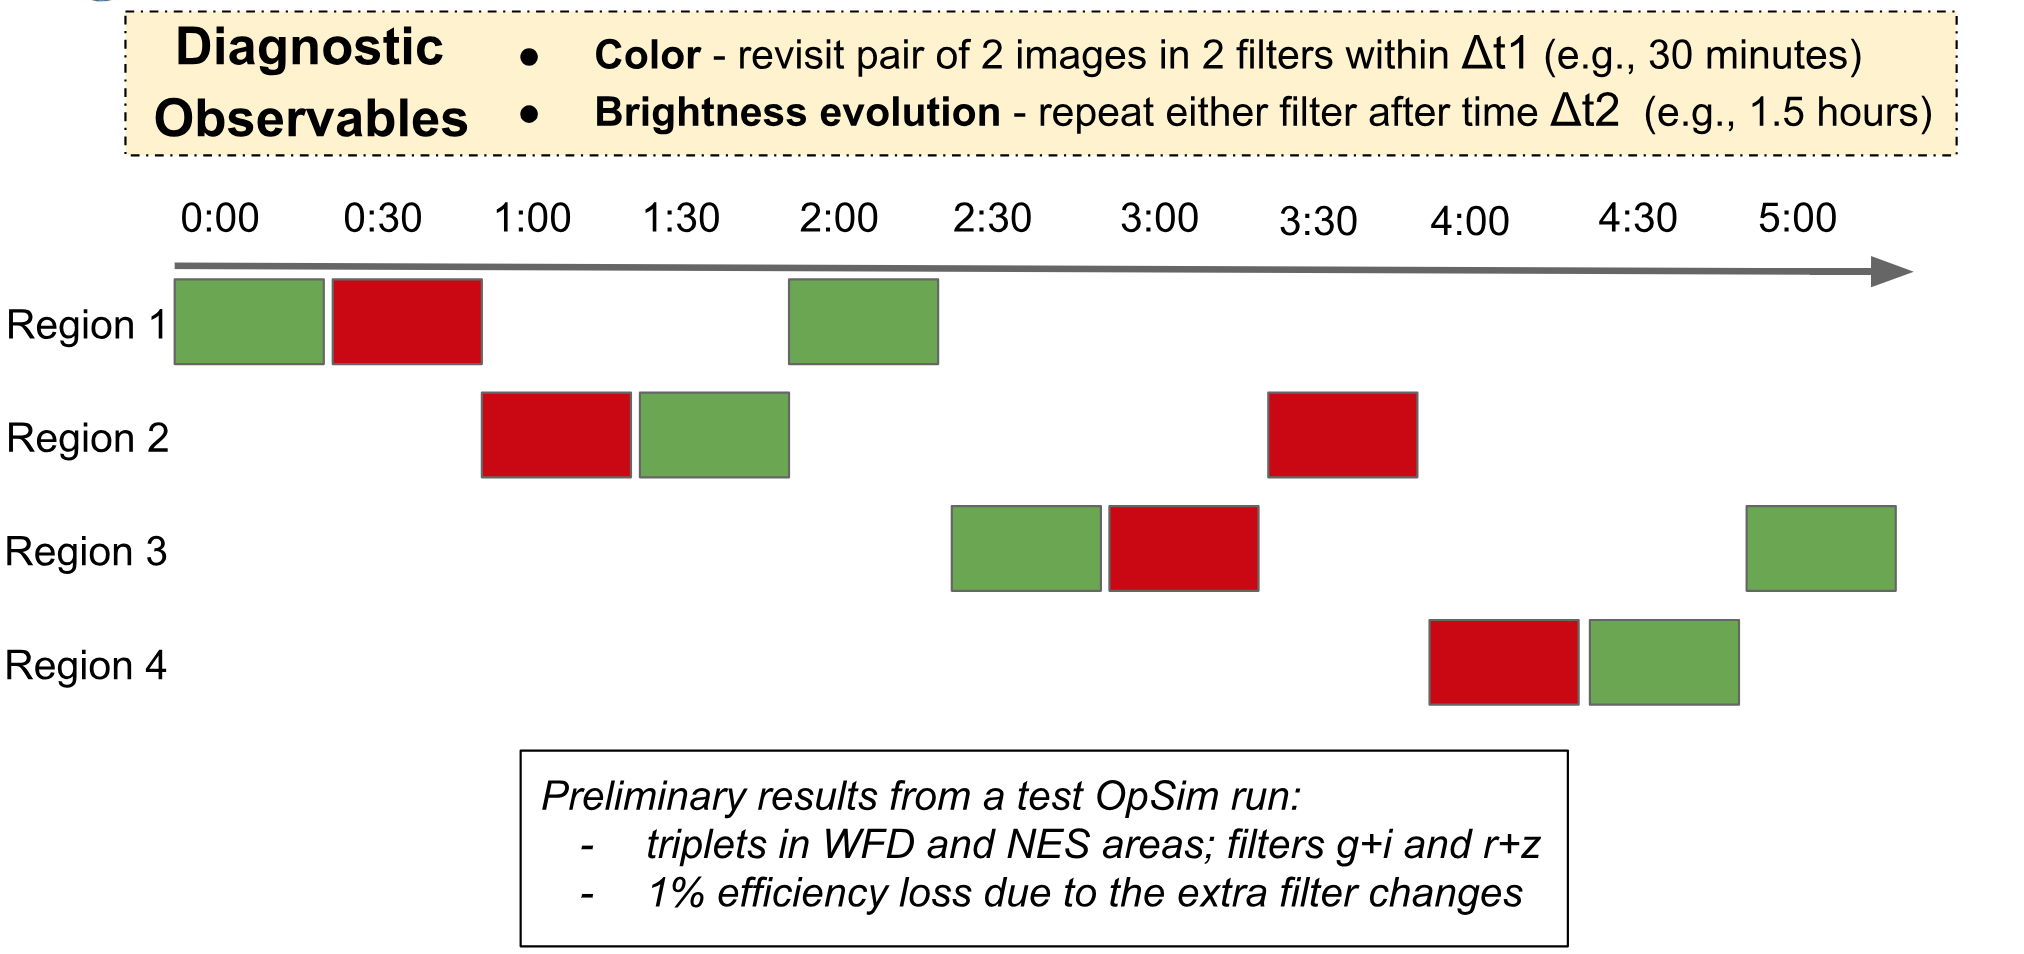
\includegraphics[width=0.9\textwidth]{figures/highLevelCadence.png}
\caption{Cadence example: two alternating filters cover regions of sky to obtain 3 observations per region, in 2 filters, with apprioriate time gaps to measure lightcurve color and shape.}
\end{figure}

\subsection{Footprint -- pointings, regions and/or constraints}
\begin{footnotesize}{\it Describe the specific pointings or general region (RA/Dec, Galactic longitude/latitude or Ecliptic longitude/latitude) for the observations. Please describe any additional requirements, especially if there are no specific constraints on the pointings (e.g. stellar density, galactic dust extinction).}
\end{footnotesize}

This proposed cadence does not make any additional constraints on the imaging area compared to WFD. The science goals might be reachable if the proposed cadence was implemented over a sub-region of the WFD survey area.  

\subsection{Image quality}
\begin{footnotesize}{\it Constraints on the image quality (seeing).}\end{footnotesize}

This proposed cadence does not make any additional constraints on the image quality compared to WFD. 

\subsection{Individual image depth and/or sky brightness}
\begin{footnotesize}{\it Constraints on the sky brightness in each image and/or individual image depth for point sources. Please differentiate between motivation for a desired sky brightness or individual image depth (as calculated for point sources). Please provide sky brightness or image depth constraints per filter.}
\end{footnotesize}

This proposed cadence does not make any additional constraints on the individual image depth or sky brightness compared to WFD. 


\subsection{Co-added image depth and/or total number of visits}
\begin{footnotesize}{\it  Constraints on the total co-added depth and/or total number of visits. Please differentiate between motivations for a given co-added depth and total number of visits. Please provide desired co-added depth and/or total number of visits per filter, if relevant.}
\end{footnotesize}

This proposed cadence does not make any additional constraints on the co-added image depth or total number of visits compared to WFD. 


\subsection{Number of visits within a night}
\begin{footnotesize}{\it Constraints on the number of exposures (or visits) in a night, especially if considering sequences of visits.}
\end{footnotesize}

The proposed candence requires at least 3 visits per night.

\subsection{Distribution of visits over time}
\begin{footnotesize}{\it Constraints on the timing of visits --- within a night, between nights, between seasons or between years (which could be relevant for rolling cadence choices in the WideFastDeep. Please describe optimum visit timing as well as acceptable limits on visit timing, and options in case of missed visits (due to weather, etc.). If this timing should include particular sequences of filters, please describe.}
\end{footnotesize}

Three observations in 2 filters, 2 in different filters separated by $\lesssim45$ minutes, returning to the field in the same night with either one of the filters in $\gtrsim90$ minutes.

We furthermore note that the science goals motivating this cadence -- namely, well-characterized light curves for rapid events -- have overlap with the science motivations of a rolling cadence. Our proposed cadence would benefit from being implemented in regions where rolling cadence is applied (i.e., an intranight gap $<3$ days).


\subsection{Filter choice}
\begin{footnotesize}
{\it Please describe any filter constraints not included above.}
\end{footnotesize}

Filters should be pair with a gap in the sequence: g-i or r-z.                                                       
\subsection{Exposure constraints}
\begin{footnotesize}
{\it Describe any constraints on the minimum or maximum exposure time per visit required (or alternatively, saturation limits). Please comment on any constraints on the number of exposures in a visit.}
\end{footnotesize}

This proposed cadence uses the baseline exposure times of $2\times15$ seconds or $1\times30$ seconds.

\subsection{Other constraints}
\begin{footnotesize}
{\it Any other constraints.}
\end{footnotesize}

We propose that this cadence be implemented on extragalactic fields, but note that it may also be useful in some Galactic Plane fields to detect and characterize microlensing events on short timescales, binary stars, and black holes, for example. Trade-offs and synergies with other proposals are discussed further in Section 3.12, Item 5.


\subsection{Estimated time requirement}
\begin{footnotesize}
{\it Approximate total time requested for these observations, using the guidelines available at \url{https://github.com/lsst-pst/survey_strategy_wp}.}
\end{footnotesize}

Since our proposed cadence is a modification of the WFD strategy -- a shuffling of the visits, not adding visits -- we are not requesting that any additional time be added to the WFD component.

\vspace{.3in}

\begin{table}[ht]
    \centering
    \begin{tabular}{l|l|l|l}
        \toprule
        Properties & Importance \hspace{.3in} \\
        \midrule
        Image quality &   3  \\
        Sky brightness &  3\\
        Individual image depth & 3  \\
        Co-added image depth &   3\\
        Number of exposures in a visit   &  3 \\
        Number of visits (in a night)  &  1 \\ 
        Total number of visits &   3\\
        Time between visits (in a night) & 1 \\
        Time between visits (between nights)  & 2  \\
        Long-term gaps between visits & 3\\
        Other \emph{filter pairs within night} & 1 \\
        \bottomrule
    \end{tabular}
    \caption{{\bf Constraint Rankings:} Summary of the relative importance of various survey strategy constraints. Please rank the importance of each of these considerations, from 1=very important, 2=somewhat important, 3=not important. If a given constraint depends on other parameters in the table, but these other parameters are not important in themselves, please only mark the final constraint as important. For example, individual image depth depends on image quality, sky brightness, and number of exposures in a visit; if your science depends on the individual image depth but not directly on the other parameters, individual image depth would be `1' and the other parameters could be marked as `3', giving us the most flexibility when determining the composition of a visit, for example.}
        \label{tab:obs_constraints}
\end{table}

\subsection{Technical trades}
{\footnotesize {\it To aid in attempts to combine this proposed survey modification with others, please address the following questions:}}
\begin{enumerate}
    \item {\footnotesize {\it What is the effect of a trade-off between your requested survey footprint (area) and requested co-added depth or number of visits?}} \\ As with a rolling cadence, the area in which this {\em Presto-Colore} strategy is applied will lower the visit cadence in other areas.
    \item {\footnotesize {\it If not requesting a specific timing of visits, what is the effect of a trade-off between the uniformity of observations and the frequency of observations in time? e.g. a `rolling cadence' increases the frequency of visits during a short time period at the cost of fewer visits the rest of the time, making the overall sampling less uniform.}} \\ As with a rolling cadence, during the time when a field is not within the area being covered by the {\em Presto-Colore} strategy, it will receive fewer visits.
    \item {\footnotesize {\it What is the effect of a trade-off on the exposure time and number of visits (e.g. increasing the individual image depth but decreasing the overall number of visits)?}} \\ Discovering and characterizing fast transients and fast features does not benefit from an increase in exposure time at the expense of the number of visits. 
    \item {\footnotesize {\it What is the effect of a trade-off between uniformity in number of visits and co-added depth? Is there any benefit to real-time exposure time optimization to obtain nearly constant single-visit limiting depth?}} \\ The science goals that motivate the {\em Presto-Colore} strategy do not benefit from increased co-added depth or maintaining a constant single-visit limiting depth.
    \item {\footnotesize {\it Are there any other potential trade-offs to consider when attempting to balance this proposal with others which may have similar but slightly different requests?}} \\ There are a few other proposals similar to the {\em Presto-Colore} strategy proposed in this white paper. \\ (1) Street et al. ``The Diverse Science Return from a Wide-Area Survey of the Galactic Plane", which proposes the ``paired-$i$" strategy: fields in the Galactic plane are imaged every 2-3 days, first in $i$-band and then 1-4 hours later a revisit in $g$, $r$, or $z$. The basic motivation is the same -- to identify rapidly varying transients and characterize them via colors -- just for Galactic variables like Young Stellar Objects and Cataclysmic Variables. However, since we propose the {\em Presto-Colore} strategy for the extragalactic WFD there is no tension between these two white papers. \\ (2) Bricman et al. ``TDEs with LSST", {\bf which proposes to change the filter between the two $15$-second exposures of a visit. MLG notes this is a 400\% overhead (120s filter change over 30s visit); surely they're going to change their proposal, so we'll write this blurb later.} \\ (3) Gezari et al. ``An Extreme Rolling Cadence Wide-Fast-Deep Survey", proposes to do the full WFD area in only years 1 and 10, and rotate through 8 equal strips of area in years 2 through 9. While this would often result in 2-3 visits per night, probably in multiple filters, no specific filter pairings or revisit timescales are requested. We would not advocate for this extreme rolling cadence as an alternative route to our science goals; for example, it would remove the opportunity for longer-term monitoring of transients with fast features, such as Type IIn SNe which can last for years. 
\end{enumerate}


\clearpage
%%%%%%%%%%%%%%%%%%%%%%%%%%%%%%%%%%%%%%%%%%%%%%%%%%%
\section{Performance Evaluation}
\begin{footnotesize}
{\it Please describe how to evaluate the performance of a given survey in achieving your desired science goals, ideally as a heuristic tied directly to the observing strategy (e.g. number of visits obtained within a window of time with a specified set of filters) with a clear link to the resulting effect on science. More complex metrics which more directly evaluate science output (e.g. number of eclipsing binaries successfully identified as a result of a given survey) are also encouraged, preferably as a secondary metric. If possible, provide threshold values for these metrics at which point your proposed science would be unsuccessful and where it reaches an ideal goal, or explain why this is not possible to quantify. While not necessary, if you have already transformed this into a MAF metric, please add a link to the code (or a PR to \href{https://github.com/lsst-nonproject/sims_maf_contrib}{sims\_maf\_contrib}) in addition to the text description. (Limit: 2 pages).}
\end{footnotesize}

\subsection{Diagnostic Metric}

Based on our evaluation of the light curves of fast transients, and the fast features of longer duration transients, we create a {\it diagnostic} metric that checks for the frequency with which the LSST observing simulation executes our desired filter-revisit cadence. 

\subsection{The Other Kind of Metric}

The metric is the fraction of events for which the color and risetime is constrained (within some accuracy). Different science cases may have different input lightcurves and different gap constraints


\subsection{Create OpSim}

{\tt OpSim} runs are being created that perform $f_1$ observations on a field, 30 min later repeat the pointing pattern in $f_2$, and 60 min later repeat the pointing pattern in $f_1$ or $f_2$, where $f_1$ and $f_2$ are $g$ and $i$, or $r$ and $z$. Non-adjacent filters are used to get a better leverage on the Spectral Energy Distribution (SED) color.

\vspace{.6in}

\clearpage
%%%%%%%%%%%%%%%%%%%%%%%%%%%%%%%%%%%%%%%%%%%%%%%%%%%
\section{Special Data Processing}
\begin{footnotesize}
{\it Describe any data processing requirements beyond the standard LSST Data Management pipelines and how these will be achieved.}
\end{footnotesize}

The science goals that motivate the proposed cadence in this white paper will not require any data processing outside of the planned Prompt and Data Release pipelines and their data products. 

%%%%%%%%%%%%%%%%%%%%%%%%%%%%%%%%%%%%%%%%%%%%%%%%%%%
\bibliographystyle{aasjournal}

\bibliography{main}

\end{document}
